\documentclass[11pt]{article}

\usepackage[a4paper,margin=1in]{geometry}
\usepackage{amsmath,amssymb,amsthm}
\usepackage{enumitem}
\usepackage{xcolor}
\usepackage{fancyhdr}
\usepackage{needspace}
\usepackage{graphicx}
\usepackage{caption}

\definecolor{courseblue}{RGB}{0,0,255}
\setlength{\parindent}{0pt}
\setlength{\parskip}{0.35em}
\setlength{\headheight}{14pt}
\pagestyle{fancy}
\fancyhf{}
\fancyfoot[C]{\thepage}
\renewcommand{\headrulewidth}{0pt}

\newcounter{problem}
\newenvironment{problem}{%
    \refstepcounter{problem}%
    \Needspace{7\baselineskip}%
    \par\vspace{0.7em}%
    \noindent\textcolor{courseblue}{\rule{\textwidth}{0.4pt}}%
    \par\vspace{0.5em}%
    \begin{list}{}{%
        \setlength{\leftmargin}{2.3em}%
        \setlength{\labelwidth}{1.8em}%
        \setlength{\labelsep}{0.5em}%
        \setlength{\topsep}{0pt}%
        \setlength{\partopsep}{0pt}%
    }%
    \item[\theproblem.]
}{\end{list}\par\vspace{0.5em}}
\newenvironment{parts}{%
    \begin{enumerate}[label=(\alph*),leftmargin=2.2em,itemsep=0.65em,topsep=0.65em]
}{\end{enumerate}}

% Type your solutions between \begin{answer} and \end{answer}.
% The answer blocks expand automatically as you add text, equations, or figures.
\newenvironment{answer}{%
    \Needspace{4\baselineskip}%
    \par\vspace{0.35em}\noindent\textbf{Answer:}\par
}{\par\vspace{1.5em}}

\begin{document}
\begin{center}
    {\color{courseblue}\Large\textbf{CS 335}\hfill\textbf{Fall 2026}}

    \vspace{1.2em}
    {\color{courseblue}\Large Assignment 1 Submission}

    Due Monday, October 5, 2026, 5:00pm

    \vspace{0.8em}
    \textbf{Name:} Vlad Paun

    \textbf{Student number:} 21291453
\end{center}

\begin{problem}
\textbf{(6 marks)} No-arbitrage option pricing.

Suppose the current price of a stock is \$18. Consider a two state tree model defined such that
after 3 months, the stock price may increase to \$19 with a 40\% probability or decrease to \$16
with a 60\% probability. Consider a European call option, based on this stock, with strike price
$K=\$17$ and expiry time $T=3$ months. Assume the risk-free interest rate is 9\%.
\begin{parts}
\item (3 marks) Construct a risk-free portfolio and use it to determine the present no-arbitrage
value (fair value) of the option (i.e., at time $t=0$).
\begin{answer}
    % Your answer here.
\end{answer}
\item (3 marks) Suppose such an option is priced on the market at $V^*=2.0$ (i.e., \emph{higher} than
the no-arbitrage price). Describe the details for a strategy that will result in a guaranteed
profit (in present value, i.e., at $t=0$) and determine the value of that profit (per option),
somewhat similar to what we did in class. (As usual in this course, we will assume short-selling
is allowed and the no-arbitrage principle holds.)
\begin{answer}
    % Your answer here.
\end{answer}
\end{parts}
\end{problem}

\begin{problem}
\textbf{(10 marks)} Coding: Convergence of a walk on a discrete lattice.

Consider a random walk on an $N$ step lattice on $t\in[0,T]$ with the parameters
\begin{align*}
X_{n+1}&\ \to\ X_n+\sigma\sqrt{\Delta t}\ ;\quad\text{with probability }p\\
X_{n+1}&\ \to\ X_n-\sigma\sqrt{\Delta t}\ ;\quad\text{with probability }1-p\\
p&=\frac12\left[1+\frac{\alpha}{\sigma}\sqrt{\Delta t}\right]\\
\Delta t&=\frac{T}{N},
\end{align*}
which converges to the solution of the SDE
\[
dX=\alpha\,dt+\sigma\,dZ,
\]
as $\Delta t\to0$. The exact solution to this SDE is such that the exact density (probability distribution)
of $X(T)$ is a normal density with mean $X_{init}+\alpha T$ and standard deviation $\sigma\sqrt{T}$,
assuming the initial value of $X$ is $X_{init}$.

Verify this experimentally via numerical simulation of many lattice walks, by preparing a
Jupyter/Python notebook to carry out the following. Perform a lattice walk simulation, using
the parameters given in Table~\ref{tab:data}. Starting at $X_0=X_{init}$, the value of $X$ is then moved up
with probability $p$ or down with probability $(1-p)$. A \emph{uniformly} distributed random number
on $[0,1]$ should be generated and used to determine the actual move taken. At the next lattice
node (i.e., time step), this process is repeated, until we obtain the final position of $X$ after $N$
steps, $X_N$, at $t=T$. This is a single simulation outcome; we perform many such simulations
to produce many (possibly) different outcomes. Because each step moves up or down a fixed
amount, the set of all possible outcomes for this discrete lattice walk is
\[
X_N^j=X_{init}+\left\{(2j-N)\sigma\sqrt{\Delta t}\right\}
\qquad j=0,\ldots,N.
\]
As indicated in Table~\ref{tab:data}, you should perform the above process first for 1000 simulations, then
separately for 10,000 simulations, and finally for 100,000 simulations. In each case, print out
the number of simulations and the corresponding mean and standard deviation of the computed
values of $X_N$ from the simulations in that set. Also, print out the anticipated exact mean and
standard deviation for comparison.

Next, for each set of simulations, we would like to generate a histogram of the observed \emph{probability
density} versus $X(T)$ as described below.

Care must be taken in scaling this histogram to get the correct probability density. Let $p(x)$ be
the probability density, and let $\operatorname{bin}_{[a,b]}$ be the bin on an interval $[a,b]$ of the $x$ axis. Then
\begin{align*}
\int_a^b p(x)\,dx&\simeq p((a+b)/2)(b-a)\\
&\simeq\frac{\text{Number of occurrences in }\operatorname{bin}_{[a,b]}}
{\text{Total number of occurrences}}
\end{align*}
so that
\[
p((a+b)/2)\simeq\frac{1}{(b-a)}
\frac{\text{Number of occurrences in }\operatorname{bin}_{[a,b]}}
{\text{Total number of occurrences}}.
\]
Use $N+1$ bins, with the bin boundaries falling half-way between the lattice nodes at timestep $N$.
Use matplotlib's \emph{bar} function to display your probability density plot constructed as described
above. (Alternatively, if you prefer, Matplotlib's \emph{hist} or Numpy's \emph{histogram} functionality can
automate some of this process, if you give it appropriately chosen values for the range, bin width,
and density parameters.) Be sure to include appropriate labeling on your plots (axis labels, title,
legend if necessary).

Then, for comparison, over top of each of your histograms, generate a standard (line) plot of
the true normal distribution with mean $X_{init}+\alpha T$ and standard deviation $\sigma\sqrt{T}$, over the same
range (in a different color). The Scipy function \texttt{stats.norm.pdf} can be used to evaluate a true
normal distribution function. Thus each of your three plots will look something roughly along
the lines of Figure~\ref{fig:example} (albeit generated with different data).

\begin{center}
% Preserve the original example plot directly from page 3 of assignment1-exercises.pdf.
% Keep assignment1-exercises.pdf beside this source when compiling.
\includegraphics[page=3,trim=178 570 180 60,clip,width=0.62\linewidth]{assignment1-exercises.pdf}
\captionof{figure}{A histogram of an approximate probability density function, with a normal distribution plotted on top.}
\label{fig:example}
\end{center}

\begin{center}
\begin{tabular}{|c|r|}
\hline
$T$ & 1.75\\
$\sigma$ & 0.3\\
$\alpha$ & 0.4\\
$X_{init}$ & 17\\
Number of simulations & 1000, 10000, 100000\\
Number of timesteps ($N$) & 300\\
\hline
\end{tabular}
\captionof{table}{\emph{Data to be used in your simulations of discrete walks on a lattice.}}
\label{tab:data}
\end{center}

Your code must be \emph{vectorized} for efficiency, i.e., prefer vector operations instead of scalar operations.
As a very simple example of vectorization, if I have a Numpy vector $V$ and I want to
add 1 to every entry of the vector, I can simply write the vector operation $V=V+1$, instead
of using a slower for loop over index $i$ and separately computing $V[i]=V[i]+1$ for each entry.
Similarly, many Numpy functions work on vectors rather than single numbers.

Specifically, your code for the lattice walk should only explicitly loop over the timesteps, not
over the individual simulations - for each time step, the updates for all the simulations (within a
set) should be computed together using vector operations. Also, you should not store the entire
lattice at once, but rather only one or two columns of it, to save on memory. The example lattice
walk code in the course notes is likely to be \emph{very helpful}, since it illustrates both vectorization
and lattice walk implementation! (Course notes, page 17).

In addition to the NumPy functions mentioned previously above, you may also find the \emph{mean},
\emph{std}, and \texttt{random.uniform} functions useful.

In a markdown cell in your Jupyter notebook, describe what you observe about your results
(plots and statistics) as the number of simulations increases from 1000 to 100,000.
\begin{answer}
    % Add your written discussion, results, and figures here.
\end{answer}
\end{problem}

\begin{problem}
\textbf{(6 marks)} Coding: Brownian motion and Ito calculus.

Let
\begin{align*}
\Delta Z_i&=\phi(t_i)\sqrt{\Delta t}\\
\phi(t_i)&\sim N(0,1)\\
Z(t_0=0)&=0\\
Z(t_i)&=\sum_{j=0}^{i-1}\Delta Z_j\\
t_i&=i\,\Delta t
\end{align*}
and
\begin{align*}
I(T,\Delta t)&=\sum_{i=0}^{N-1}(\Delta Z_i)^2\\
\Delta t&=\frac{T}{N}.
\end{align*}
Write a Jupyter/Python notebook to evaluate $I(T,\Delta t)$. For $T=2$, for fixed $\Delta t$, compute the
value of $I(T,\Delta t)$. Use 70000 paths, and compute the mean and variance of the result, for $N=$
100, 200, 400, 800, 1600, 3200, 6400 timesteps. Vectorize your code so that there is only one
explicit for loop over the timesteps, for a given value of $N$.

Write code to generate a simple text-based table of mean and variance of $I(T,\Delta t)$ for the different
values of $\Delta t$. (No fancy formatting is required! You can just use Python's print function to
generate each row, with appropriate arguments.)

Plot a graph of $\operatorname{var}(I(T,\Delta t))$ versus $\Delta t$, with appropriate labels. In a markdown cell of your
Jupyter notebook, explain mathematically what you observe.
\begin{answer}
    % Add your written discussion, results, and figures here.
\end{answer}
\end{problem}

\begin{problem}
\textbf{(5 marks)} Ito calculus.
\begin{parts}
\item (3 marks) Let $X(t)$ and $Y(t)$ be two stochastic processes, such that
\begin{align*}
dX&=\mu_X(X(t),t)dt+\sigma_X(X(t),t)dZ_X\\
dY&=\mu_Y(Y(t),t)dt+\sigma_Y(Y(t),t)dZ_Y
\end{align*}
with $dZ_X(t)$, $dZ_Y(t)$ being the increments for two distinct Wiener processes, $Z_X(t)$ and $Z_Y(t)$.
Let $X(t_i)=X_i$ and $Y(t_i)=Y_i$. Show that
\begin{align*}
(X_{i+1}-X_i)(Y_{i+1}-Y_i)
&=X_{i+1}Y_{i+1}-X_iY_i\\
&\quad-X_i(Y_{i+1}-Y_i)-Y_i(X_{i+1}-X_i).
\end{align*}
\Needspace{9\baselineskip}
Then, using the definition of the Ito integral which is the limit of a discrete sum, show that
\[
\int_0^t X(s)dY(s)=[XY]_0^t-\int_0^t Y(s)dX(s)-\int_0^t dX(s)dY(s).
\]
\begin{answer}
    % Your answer here.
\end{answer}
\item (2 marks) Let $Z(t)$ be a stochastic process satisfying $dZ=\phi\sqrt{dt}$, and assume $Z(0)=0$.
Using the result in part (a), show that (assuming Ito calculus)
\[
\int_0^t Z(s)\,dZ(s)=\frac12 Z(t)^2-\frac{t}{2}.
\]
\begin{answer}
    % Your answer here.
\end{answer}
\end{parts}
\end{problem}

\begin{problem}
\textbf{(10 marks)} Ito calculus and Ito's Lemma.

Suppose $dZ$ is the increment of a Wiener process and
\[
dX=\mu(X(t),t)dt+\sigma(X(t),t)dZ.
\]
\begin{parts}
\item (6 marks) If
\[
F(X,t)=X^4e^{-t}+3X\cos t,
\]
what is $dF(X,t)$ (interpreted in the sense of Ito calculus)?
\begin{answer}
    % Your answer here.
\end{answer}
\item (4 marks) Using $dX$ as defined above, and expanding, simplify
\[
\int_0^T(dX)^2
\]
as much as possible. The integral is to be interpreted in the Ito calculus sense. (Note that
$\sigma(X(t),t)$ is a function of $t$, not a constant, so you will not be able to fully solve the integral.)
\begin{answer}
    % Your answer here.
\end{answer}
\end{parts}
\end{problem}
\end{document}
